\section{Background and fundamentals}\label{sec:bg}

This section defines every concept that the rest of the supplement uses, starting from how images are sampled and building up to the neural networks, the frame-time budget and the metrics. Each concept is defined before it is used, and each symbol is defined where it first appears. The code files named here are in \texttt{src/neuralss}. Where the code computes a quantity in a convention that differs from the textbook one, the text states the code's convention, and the code is the reference for every definition in this section.

A frame at time index $t$ is written $I_t$, a function from pixel positions to RGB values in $[0,1]^3$. A pixel position is $\mathbf p=(x,y)$ in pixel units, with $x$ the column and $y$ the row, and the code indexes integer positions in the same way. The scale factor $s$ is the ratio of the output to the input linear size, so a low-resolution frame of $h\times w$ pixels is upscaled to $sh\times sw$ pixels.

\subsection{Digital images}\label{sec:bg-images}

A digital image is a finite array of samples. A frame of $H\times W$ pixels with three colour channels is stored as floating-point values in $[0,1]$, and 8-bit files are divided by 255. Three properties of such an array matter for everything that follows: how its values are encoded, how its luminance is measured and how many pixels it has.

\paragraph{Encoding and linear light.} Stored display values are gamma encoded, so they are not proportional to the light $L$ that the display emits. The sRGB transfer curve, implemented by \texttt{srgb\_to\_linear} and \texttt{linear\_to\_srgb} in \texttt{nss\_synth.py}, converts between an encoded value $E\in[0,1]$ and a linear light value $L\in[0,1]$:
\begin{align}
L&=\begin{cases}E/12.92, & E\le 0.04045,\\ \big((E+0.055)/1.055\big)^{2.4}, & E>0.04045,\end{cases}\label{eq:bg-srgb}\\
E&=\begin{cases}12.92\,L, & L\le 0.0031308,\\ 1.055\,L^{1/2.4}-0.055, & L>0.0031308.\end{cases}\nonumber
\end{align}
Light adds in linear values, so an average of light must be taken after decoding. The synthetic renderer decodes its shading, multiplies by the exposure and encodes again. Its four-sample supersampling, however, averages values that are already encoded, so the synthetic targets are not exact linear-light averages. All metrics in this supplement compare encoded values as stored, which is the usual convention for image quality measures and not a measurement of linear-light error.

\paragraph{Luma.} The code measures luminance as the studio-range luma of the encoded values,
\begin{equation}
Y=\frac{16+65.481\,R+128.553\,G+24.966\,B}{255}=\frac{16}{255}+\frac{219}{255}\big(0.299\,R+0.587\,G+0.114\,B\big),\label{eq:bg-luma}
\end{equation}
where $R,G,B\in[0,1]$ and the two forms are identical (\texttt{rgb\_to\_y}). The second form shows that $Y$ is an affine function of the full-range luma $0.299R+0.587G+0.114B$. A white pixel gives $Y=235/255\approx0.92$ and a black pixel gives $Y=16/255\approx0.06$, so $Y$ spans $[0.06,0.92]$ rather than $[0,1]$. Every luma-based measure in the supplement uses Eq.~(\ref{eq:bg-luma}): PSNR-Y, SSIM on luma, the luma gradient mask of the detail region and the cut detector. The defect test (\texttt{clip\_defects}) and the census loss use the full-range form without the affine map. The weights $0.299$, $0.587$ and $0.114$ are the ITU-R BT.601 luma weights, which are a standard rather than a journal article.\footnote{Recommendation ITU-R BT.601-7, \url{https://www.itu.int/rec/R-REC-BT.601}, accessed 9 November 2026.}

\paragraph{YCoCg.} The analytic temporal upscaler clamps its history in the YCoCg space,
\begin{equation}
Y=\tfrac14R+\tfrac12G+\tfrac14B,\qquad C_o=\tfrac12R-\tfrac12B,\qquad C_g=-\tfrac14R+\tfrac12G-\tfrac14B,\label{eq:bg-ycocg}
\end{equation}
with the inverse $R=Y+C_o-C_g$, $G=Y+C_g$ and $B=Y-C_o-C_g$. The transform is invertible, so a round trip is exact up to rounding. The $Y$ of Eq.~(\ref{eq:bg-ycocg}) is a green-weighted average of the channels and is a different quantity from the luma of Eq.~(\ref{eq:bg-luma}), which shares only its name. The code's functions are \texttt{rgb\_to\_ycocg} and \texttt{ycocg\_to\_rgb}.

\paragraph{Resolution and scale.} A frame of $H\times W$ pixels has $HW$ pixels. In this supplement, 1080p means $1920\times1080$ pixels, which is $2{,}073{,}600$ pixels with a 16:9 aspect ratio, unless a different size is stated. An upscaler at scale $s$ maps $h\times w$ pixels to $sh\times sw$. Producing one 1080p output at scale $s$ therefore requires $(1920/s)\times(1080/s)$ low-resolution pixels, which is $640\times360=230{,}400$ for $s=3$ and $960\times540=518{,}400$ for $s=2$. The notebooks time configurations from $640\times360$ to $1920\times1080$ at 3x, from $960\times540$ to $1920\times1080$ at 2x and from $1280\times720$ to $3840\times2160$ at 3x. The render resolution is the low-resolution size of the upscaler's input, and the output resolution is the display size.

\subsection{Sampling, aliasing and jitter}\label{sec:bg-sampling}

\paragraph{Sampling.} A renderer evaluates a continuous scene $f(\mathbf q)$ at positions $\mathbf q\in\mathbb R^2$ and writes one value per pixel. The ideal value of pixel $i$ is the average of the scene over the pixel's area $A_i$,
\begin{equation}
P_i=\frac{1}{|A_i|}\int_{A_i}f(\mathbf q)\,\mathrm d\mathbf q,\label{eq:bg-area}
\end{equation}
which filters the scene with a box. A renderer that takes one point sample per pixel, $P_i\approx f(\mathbf c_i)$ at the pixel centre $\mathbf c_i$, does not filter. The synthetic renderer (\texttt{Scene.frame}) draws low-resolution frames with one bilinear sample of each texture per pixel and without mip filtering, so thin geometry is point-sampled and aliases. Real clips receive the same treatment when they become low-resolution inputs: \texttt{\_sr\_inputs} bilinearly samples the full-resolution frame at the sample positions, unless the clip supplies native low-resolution frames.

\paragraph{Nyquist and aliasing.} A signal sampled at $f_s$ samples per unit length can represent frequencies up to the Nyquist frequency $f_s/2$, and no higher.\cite{shannon1949communication} Content above the Nyquist frequency does not disappear. It is folded into the representable band, so a sinusoid of frequency $f$, sampled at multiples of the sample spacing, cannot be told apart from one of frequency
\begin{equation}
f_a=\left|f-k f_s\right|,\qquad k=\operatorname{round}(f/f_s),\label{eq:bg-alias}
\end{equation}
which lies in $[0,f_s/2]$. As a worked example, take one sample per pixel and stripes with a period of 1.5 pixels, which have $f=2/3$ cycles per pixel. That is above the Nyquist frequency of $1/2$ cycle per pixel. At the pixel centres $n\in\mathbb Z$,
\begin{align*}
\cos\!\Big(2\pi\cdot\tfrac23\,n\Big)&=\cos\!\Big(2\pi n-\tfrac{2\pi n}{3}\Big)\\
&=\cos\!\Big(\tfrac{2\pi n}{3}\Big),
\end{align*}
which is a sinusoid of frequency $f_a=|2/3-1|=1/3$, a period of 3 pixels. The 1.5-pixel stripes therefore appear as 3-pixel stripes with a different phase. Thin geometry behaves the same way in time. A wire one texel wide that moves by a fraction of a pixel per frame is hit by the sample in some pixels and missed in others, and the set of hit pixels changes from frame to frame. The result is flicker, which a supersampled target for the same frame does not show.

\paragraph{Supersampling.} Averaging $K$ point samples per pixel approximates Eq.~(\ref{eq:bg-area}),
\begin{equation}
P_i\approx\frac1K\sum_{k=1}^{K}f(\mathbf c_i+\mathbf o_k),\label{eq:bg-ssaa}
\end{equation}
where $\mathbf o_k$ are sample offsets inside the pixel. The renderer's targets use $K=4$ at output resolution with the offsets $(-0.375,-0.125)$, $(0.125,-0.375)$, $(0.375,0.125)$ and $(-0.125,0.375)$ in pixel units, which form a rotated grid (\texttt{SSAA\_OFFSETS}). As noted above, these four values are averaged after encoding.

\paragraph{Sub-pixel jitter.} Rendering $K$ samples per pixel costs $K$ times as much as one. A cheaper alternative takes one sample per pixel per frame and moves the sample grid by a different sub-pixel offset $\mathbf j_t$ in each frame, so the samples of successive frames fall at different places inside each pixel. The offsets are measured in pixels of the low-resolution grid and lie in $[-0.5,0.5)^2$. \Cref{fig:bg-jitter} shows the sample positions of two consecutive frames.

\begin{figure}[!htbp]
\centering
\begin{tikzpicture}[scale=1.25]
  \foreach \k in {0,...,9}{
    \draw[gray!25] (\k/3,-3) -- (\k/3,0);
    \draw[gray!25] (0,-\k/3) -- (3,-\k/3);
  }
  \draw[gray!70, thick] (0,-3) grid (3,0);
  \foreach \i in {0,1,2}{
    \foreach \j in {0,1,2}{
      \fill[gray] (\i+0.5,-\j-0.5) circle (1.1pt);
      \fill[blue!70!black] (\i+0.5,-\j-0.5+0.1667) circle (1.9pt);
      \draw[red!70!black, thick] (\i+0.25-0.06,-\j-0.6667-0.06) -- (\i+0.25+0.06,-\j-0.6667+0.06);
      \draw[red!70!black, thick] (\i+0.25-0.06,-\j-0.6667+0.06) -- (\i+0.25+0.06,-\j-0.6667-0.06);
    }
  }
  \node[anchor=south, font=\footnotesize] at (1.5,0.1) {low-resolution pixels (grey lines), output pixels at 3x (faint lines)};
  \node[anchor=west, font=\footnotesize] at (3.15,-0.35) {frame $0$: dots};
  \node[anchor=west, font=\footnotesize] at (3.15,-0.75) {frame $1$: crosses};
  \node[anchor=west, font=\footnotesize] at (3.15,-1.15) {$\mathbf j_0=(0,-\tfrac16)$};
  \node[anchor=west, font=\footnotesize] at (3.15,-1.55) {$\mathbf j_1=(-\tfrac14,\tfrac16)$};
\end{tikzpicture}
\caption{Sample positions of two consecutive frames inside a $3\times3$ patch of low-resolution pixels, with rows increasing downwards as in the code. Grey dots mark the pixel centres. Blue dots are the samples of frame $0$ and red crosses those of frame $1$, shifted by the first two Halton offsets of \cref{tab:bg-halton}. Faint lines mark the output pixels at 3x, which at this scale subdivide each low-resolution pixel into nine cells.}\label{fig:bg-jitter}
\end{figure}

\paragraph{Halton sequence.} The offsets come from the Halton $(2,3)$ sequence, a low-discrepancy sequence whose points spread evenly over the unit square with fewer large gaps than random points.\cite{halton1960efficiency} For an integer $n\ge1$ with base-$b$ digits $n=\sum_k d_k(n)\,b^k$, the radical inverse is
\begin{equation}
\varphi_b(n)=\sum_{k\ge0}d_k(n)\,b^{-(k+1)}.\label{eq:bg-halton}
\end{equation}
For example, $3=11_2$ gives $\varphi_2(3)=\tfrac12+\tfrac14=\tfrac34$, and $3=10_3$ gives $\varphi_3(3)=\tfrac19$. The function \texttt{halton} computes this by repeated division by the base. Frame $t$ uses the index $n_t=(t\bmod16)+1$ and the offset
\begin{equation}
\mathbf j_t=\big(\varphi_2(n_t)-\tfrac12,\ \varphi_3(n_t)-\tfrac12\big),\label{eq:bg-jitter}
\end{equation}
so the sequence repeats every 16 frames. The index starts at 1 because index 0 would give the corner $(-0.5,-0.5)$. Training gives each sample a random starting point in the cycle. \Cref{tab:bg-halton} lists the first four offsets, which \texttt{jitter\_sequence} produces.

\begin{table}[!htbp]
\caption{First four Halton jitter offsets. Frame $t$ uses index $n=(t\bmod16)+1$, and the offset $\mathbf j_t$ of Eq.~(\ref{eq:bg-jitter}) is in low-resolution pixels. The values were printed by \texttt{jitter\_sequence} and are rounded to three decimals}\label{tab:bg-halton}
\begin{tabular*}{\columnwidth}{@{\extracolsep\fill}rrrrrr}
\toprule
Frame $t$ & $n$ & $\varphi_2(n)$ & $\varphi_3(n)$ & $j_x$ & $j_y$ \\
\midrule
0 & 1 & $0.500$ & $0.333$ & $0.000$ & $-0.167$ \\
1 & 2 & $0.250$ & $0.667$ & $-0.250$ & $0.167$ \\
2 & 3 & $0.750$ & $0.111$ & $0.250$ & $-0.389$ \\
3 & 4 & $0.125$ & $0.444$ & $-0.375$ & $-0.056$ \\
\botrule
\end{tabular*}
\end{table}

\paragraph{Why jitter and accumulation recover resolution.} Take a static scene and one jittered sample per low-resolution pixel per frame. If the samples of earlier frames are placed at their true positions, using each frame's known offset, then after $N$ frames each low-resolution pixel holds $N$ samples at $N$ different positions. The output needs $s^2$ pixels per low-resolution pixel, so the samples must cover the $s^2$ sub-cells, and the Halton positions do this within a few frames. Jitter-aware upsampling does the placement: it samples the low-resolution frame at the output pixel centre minus the jitter (\texttt{jitter\_upsample}), so each sample lands at its true position.

Accumulation is a weighted average. Consider an exponential average $\hat y=\sum_{k\ge0}w_kx_{t-k}$ with weights $w_k=\alpha(1-\alpha)^k$, $0<\alpha\le1$, which sum to one. For samples $x_{t-k}$ with independent noise of variance $\sigma^2$,
\begin{equation}
\operatorname{Var}\hat y=\sum_{k\ge0}w_k^2\sigma^2=\frac{\alpha^2\sigma^2}{1-(1-\alpha)^2}=\frac{\alpha}{2-\alpha}\,\sigma^2,
\end{equation}
so the average behaves like a mean of $N_{\text{eff}}=(2-\alpha)/\alpha$ independent samples. For $\alpha=0.1$, the blend used by the analytic baseline of \cref{sec:bg-taa}, $N_{\text{eff}}=19$. This holds only when the history is aligned, so that a sample from an earlier frame belongs to the same surface point, and when the content is static. Motion and disocclusion break both conditions, which is why the next subsections need reprojection and rejection.

\subsection{Motion vectors and optical flow}\label{sec:bg-motion}

\paragraph{Flow.} For frames $t$ and $s$, the flow $F_{t\to s}$ is a field of displacements in pixels. For a pixel $\mathbf p$ of frame $t$, the point $\mathbf p+F_{t\to s}(\mathbf p)$ is the position in frame $s$ of the surface point that $\mathbf p$ shows in frame $t$. The code uses the backward convention for warping, in which the field is defined on the grid of the frame being produced, $t$, and points into the source frame $s$. Frame $t$ is then predicted from frame $s$ by
\begin{equation}
\hat I_t(\mathbf p)=I_s\big(\mathbf p+F_{t\to s}(\mathbf p)\big),\label{eq:bg-flow}
\end{equation}
which is the backward warp of \cref{sec:bg-warp}. A forward flow $F_{s\to t}$ is defined on the grid of the source frame and points forward. Datasets often store forward flow, and warping with it needs a scatter step that leaves holes and overlaps, so the code converts or reverses the flow instead. The code uses these conventions:
\begin{itemize}
\item Temporal super-resolution: the motion vector of frame $t$ is $m_t=F_{t\to t-1}$, the displacement from the current frame to the previous one, at low-resolution pixels (\texttt{sr\_batch}, \texttt{raft\_mv\_and\_valid}).
\item Frame generation: the engine motion vector of the newest real frame is $M_1=F_{1\to0}$, the displacement from $I_1$ to $I_0$ (\texttt{fg\_batch}).
\item Frame generation: the intermediate flows are $F_{\tau\to0}$ and $F_{\tau\to1}$, the outputs of \texttt{IFNet} (\cref{sec:bg-interp}).
\item Exact sources: the loader plays clips with forward flow backwards (\texttt{load\_clip}). The stored flow from frame $i$ to frame $i+1$ then becomes the displacement from the later frame to the earlier one, which is the convention of $m_t$, without any inversion.
\end{itemize}

\paragraph{Engine vectors and colour flow.} An engine writes a motion vector per pixel from the transforms of the geometry it draws. The vector is exact for opaque surfaces that the engine transforms, and particles and other effects without a transform get none, which is why engines also write a reactive mask. Research systems use such engine buffers, including motion vectors, as network inputs.\cite{xiao2020nsrr} Colour-only flow estimates motion from the images. It works on any video, but it is an estimate that can be wrong at boundaries, and it cannot separate motion from a change of lighting or from an overlay that moves independently. The code uses torchvision's RAFT-Small \cite{teed2020raft} with 12 updates (\texttt{load\_raft}, \texttt{raft\_flow}), as the teacher for motion labels on real video and for tOF. The built-in motion estimator of the temporal super-resolution network is an IFNet \cite{huang2022rife}.

\paragraph{Forward-backward consistency.} For two frames $a$ and $b$ with flows $F_{a\to b}$ and $F_{b\to a}$, a pixel passes the round-trip test when
\begin{equation}
\big\|F_{a\to b}(\mathbf p)+F_{b\to a}\big(\mathbf p+F_{a\to b}(\mathbf p)\big)\big\|<1+0.05\,\big\|F_{a\to b}(\mathbf p)\big\|,\label{eq:bg-fb}
\end{equation}
which says that going to frame $b$ and back returns to the start within one pixel plus 5 percent of the flow. The code's \texttt{raft\_mv\_and\_valid} applies this test with $a$ the current frame and marks the pixels that pass as valid. Pixels that fail lie at occlusions, at disocclusions and where the flow estimate is poor.

\paragraph{Occlusion and disocclusion.} A surface point is disoccluded in frame $t$ when it is visible in $t$ but absent from the previous frame $s$, and it is occluded when it is visible in $s$ but covered in $t$. The warp of Eq.~(\ref{eq:bg-flow}) has no correct source for a disoccluded pixel, so history must not be used there. The code's validity mask $v$ equals 1 where the pixel of frame $t$ is visible in the previous frame, so $1-v$ marks the disoccluded pixels (\texttt{load\_valid}). The temporal super-resolution network also uses a depth cue, $|d_t-\mathcal W(d_{t-1})|/(|d_t|+10^{-3})$, clipped to $[0,1]$, as an input feature (\texttt{TSRNet.forward}).

\paragraph{Scene cuts.} A cut is a change of content between consecutive frames. No point corresponds across it, so any flow is meaningless, and no frame can be predicted from the one before. The code detects cuts with the distance between normalised 32-bin histograms of the luma (\texttt{cut\_score}),
\begin{equation}
d_{\text{hist}}(I_0,I_1)=\tfrac12\sum_{b=1}^{32}\big|h_0(b)-h_1(b)\big|,\label{eq:bg-cut}
\end{equation}
where $h_0$ and $h_1$ are the normalised histograms of the two frames. This distance lies in $[0,1]$ and is the total-variation distance between the two histograms. When the motion vector $M_1$ is available, the score adds $2\,\overline{|I_1-\mathcal W(I_0,M_1)|}$, twice the mean motion-compensated difference. A score above a threshold is a cut.

\subsection{Warping, reprojection and history accumulation}\label{sec:bg-warp}

\paragraph{Backward warping.} Given a frame $I$ and a flow $F$, the warp $\mathcal W(I,F)(\mathbf p)=I(\mathbf p+F(\mathbf p))$ must be evaluated at non-integer positions. The code uses bilinear interpolation. For $\mathbf q=\mathbf p+F(\mathbf p)$ with integer part $(x_0,y_0)$ and fractional parts $a=q_x-x_0$ and $b=q_y-y_0$,
\begin{equation}\begin{split}
I(\mathbf q)&=(1-a)(1-b)\,I(x_0,y_0)+a(1-b)\,I(x_0+1,y_0)\\
&\quad+(1-a)b\,I(x_0,y_0+1)+ab\,I(x_0+1,y_0+1).
\end{split}\label{eq:bg-warp}\end{equation}
The four weights are non-negative and sum to one. Positions outside the frame are clamped to the border. Backward warping gathers each output pixel from one source location, so the output has no holes or overlaps, which forward splatting cannot guarantee. \texttt{backward\_warp} implements Eq.~(\ref{eq:bg-warp}) with \texttt{grid\_sample}, using the coordinate mapping of RIFE, in which pixel index $i$ corresponds to the normalised coordinate $-1+2i/(W-1)$. \Cref{fig:bg-warp} shows one pixel.

\begin{figure}[!htbp]
\centering
\begin{tikzpicture}[scale=2.1, font=\footnotesize]
  \draw[gray!50] (-0.4,-2.4) grid (3.4,0.4);
  \foreach \i in {0,...,3}{\foreach \j in {0,...,2}{\fill[gray] (\i,-\j) circle (1.3pt);}}
  \fill[blue!12] (2,-2) rectangle (3,-1);
  \draw[blue!70!black, thick] (0.9,-0.9) rectangle (1.1,-1.1);
  \node[anchor=north east, text=blue!70!black] at (0.9,-1.1) {$\mathbf p$};
  \draw[-{Stealth[length=2mm]}, thick, dashed] (1,-1) -- (2.3,-1.6);
  \node[anchor=south, font=\scriptsize] at (1.65,-1.27) {$F_{t\to s}(\mathbf p)$};
  \fill[red!70!black] (2.3,-1.6) circle (2.2pt);
  \node[anchor=south west, text=red!70!black] at (2.3,-1.6) {$\mathbf q$};
  \node[anchor=north west] at (2.04,-1.06) {\scriptsize $0.28$};
  \node[anchor=north east] at (2.96,-1.06) {\scriptsize $0.12$};
  \node[anchor=south west] at (2.04,-1.94) {\scriptsize $0.42$};
  \node[anchor=south east] at (2.96,-1.94) {\scriptsize $0.18$};
  \node[anchor=west] at (3.6,-1.0) {\scriptsize Frame $s$ pixels (dots)};
  \node[anchor=west] at (3.6,-1.5) {\scriptsize Shaded: the four pixels};
  \node[anchor=west] at (3.6,-1.85) {\scriptsize used for $\mathbf q$, $a=0.3$, $b=0.6$};
\end{tikzpicture}
\caption{Backward warp of one pixel. Pixel $\mathbf p=(1,1)$ of frame $t$ takes the value at $\mathbf q=\mathbf p+F_{t\to s}(\mathbf p)=(2.3,1.6)$ in frame $s$. That value is the bilinear mixture of the four surrounding pixels of frame $s$, with the weights shown from Eq.~(\ref{eq:bg-warp}). The flow is illustrative.}\label{fig:bg-warp}
\end{figure}

\paragraph{Half-pixel attenuation.} Bilinear interpolation is a low-pass filter. For a shift of half a pixel the weights are $(\tfrac12,\tfrac12)$, and the frequency response at angular frequency $\omega$ radians per pixel is $\tfrac12(1+e^{-i\omega})$, whose magnitude is $|\cos(\omega/2)|$. At $\omega=\pi/2$ this is $\cos(\pi/4)\approx0.71$, and at the Nyquist frequency $\omega=\pi$ it is zero. Each warp at a fractional offset removes part of the high-frequency content. A recurrent network that warps its output every frame loses high frequencies at every step unless its residual path adds them back.

\paragraph{Reprojection and accumulation.} Reprojection moves a stored result to the current frame. A history image $H$ from frame $t-1$ becomes $H_t(\mathbf p)=\mathcal W(H,m_t)(\mathbf p)$ with $m_t=F_{t\to t-1}$, and accumulation then combines $H_t$ with the new samples. The recurrent state of the temporal super-resolution network, its output and its hidden feature map, is reprojected in the same way with the low-resolution vectors. A pixel whose motion is wrong, or which is disoccluded, takes its history from the wrong surface, and that is the source of the ghosting described in \cref{sec:bg-taa}.

\subsection{Temporal anti-aliasing and temporal upscaling}\label{sec:bg-taa}

Temporal anti-aliasing (TAA) \cite{yang2020taasurvey} combines jittered samples over time with a history buffer. For each frame it renders with a jittered sample grid, reprojects the history with motion vectors, clamps the reprojected history to the range of the current samples in a small neighbourhood, and blends the clamped history with the current samples. Temporal upscaling runs the same loop at a lower render resolution, with the accumulation buffer at output resolution.

\paragraph{Exponential blending.} Without reprojection and clamping, accumulation is $\hat y_t=\alpha x_t+(1-\alpha)\hat y_{t-1}$, where $x_t$ is the current sample value and $0<\alpha\le1$. Unrolling gives
\begin{equation}
\hat y_t=\sum_{k=0}^{t-1}\alpha(1-\alpha)^k\,x_{t-k}+(1-\alpha)^t\,\hat y_0,\label{eq:bg-ema-unroll}
\end{equation}
so the sample $k$ frames old has weight $\alpha(1-\alpha)^k$, and the initial value keeps the weight $(1-\alpha)^t$. \Cref{fig:bg-ema} shows these weights for $\alpha=0.1$. A sample 10 frames old has weight $0.035$, and the initial value still has weight $0.12$ after 20 frames.

\begin{figure}[!htbp]
\centering
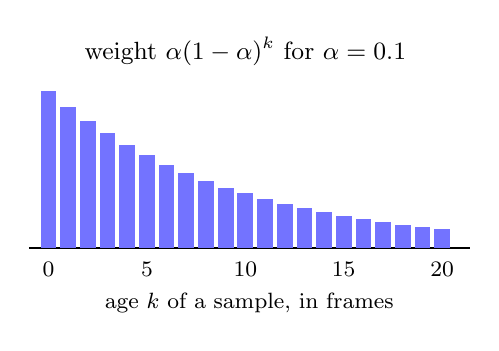
\begin{tikzpicture}[x=0.5cm, font=\footnotesize]
  \draw[thick] (-0.3,0) -- (10.9,0);
  \foreach \k/\h in {0/2.00,1/1.80,2/1.62,3/1.46,4/1.31,5/1.18,6/1.06,7/0.96,8/0.86,9/0.77,10/0.70,11/0.63,12/0.56,13/0.51,14/0.46,15/0.41,16/0.37,17/0.33,18/0.30,19/0.27,20/0.24}{
    \fill[blue!55] (\k*0.5,0) rectangle (\k*0.5+0.4,\h);
  }
  \foreach \k in {0,5,10,15,20}{
    \node[below] at (\k*0.5+0.2,-0.05) {\k};
  }
  \node[below] at (5.3,-0.45) {age $k$ of a sample, in frames};
  \node[above] at (5.2,2.2) {\small weight $\alpha(1-\alpha)^k$ for $\alpha=0.1$};
\end{tikzpicture}
\caption{Weight of a sample $k$ frames old in the exponential average of \cref{eq:bg-ema-unroll} with $\alpha=0.1$. The bar height is the weight times 20, in centimetres of the drawing. The weights fall geometrically, so an old surface that stays in the history fades slowly, which is the ghosting trail that clamping limits.}\label{fig:bg-ema}
\end{figure}

\paragraph{Ghosting.} When a surface changes, because it is disoccluded, because its motion vector is wrong or because an object leaves a region, the history still holds the old surface. That surface keeps the weight $(1-\alpha)^k$ for $k$ frames and appears as a trail behind moving objects. Clamping limits the trail. The reprojected value is confined to the range of the current neighbourhood, so an old colour far from the new samples is pulled back to the range boundary. Ghosting remains when the old colour lies inside that range, which happens when a surface and its background have similar colours. A larger $\alpha$ reduces ghosting but also reduces the averaging that removes aliasing, and that trade-off is the central design choice of TAA.

\paragraph{Analytic baseline.} The analytic upscaler of the evaluation (\texttt{AnalyticTAAU} in \texttt{nss\_metrics.py}, run by \texttt{run\_taau} in \texttt{nss\_eval.py}) implements the loop with fixed rules and stands in for analytic TAA upscalers without their proprietary heuristics. For frame $t$, with low-resolution colour $x_t$, jitter $\mathbf j_t$ and low-resolution motion vector $m_t$, it performs the following steps.
\begin{enumerate}
\item Base image: $B_t(\mathbf p)$ is the bilinear interpolation of $x_t$ at the low-resolution position of the output pixel centre $\mathbf p$ minus $\mathbf j_t$, so each sample is placed at its true position.
\item If there is no history, the output is $B_t$.
\item History: $H_t=\mathcal W\big(\hat y_{t-1},\,s\,U(m_t)\big)$, where $U$ is bilinear upsampling by $s$ and the factor $s$ converts low-resolution displacements into output pixels.
\item Clamp: with $lo$ and $hi$ the channel-wise minimum and maximum of YCoCg$(B_t)$ over the $3\times3$ output neighbourhood of each pixel, the history is clamped in YCoCg to the box between $lo$ and $hi$, and $H'_t$ is the RGB value of the clamped history.
\item Blend: $\hat y_t=H'_t+0.1\,(B_t-H'_t)$, which is 90 percent history and 10 percent current base image.
\end{enumerate}
The displayed output is clamped to $[0,1]$, but the unclamped value becomes the next history. Step 5 gives
\begin{equation}
\hat y_t=0.9\,H'_t+0.1\,B_t.\label{eq:bg-taa}
\end{equation}

Two properties of this baseline matter for the comparison. First, its docstring says that it resets on invalid history, but the code has no validity test, so every frame reprojects and clamps the history and no disocclusion rejection takes place. Second, the motion vectors are sampled at the jittered sample positions (\texttt{\_sr\_inputs}), while the baseline interprets low-resolution vectors as if they were at the pixel centres. The resulting error is the jitter times the local gradient of the motion field, which vanishes for uniform motion and is largest at motion boundaries. The temporal super-resolution network receives the same low-resolution vectors and interprets them in the same way. The supplement describes these properties as they are in the code.

\subsection{Neural building blocks}\label{sec:bg-cnn}

The networks use a small set of operators. Each is defined here with the code's convention and with the reason for its use.

\paragraph{Convolution and multiply-accumulates.} A convolutional layer with $C_{\text{in}}$ input channels, $C_{\text{out}}$ output channels and a $k\times k$ kernel $K$ computes, with stride 1 and padding $(k-1)/2$,
\begin{equation}
Y[o,i,j]=b_o+\sum_{c=1}^{C_{\text{in}}}\sum_{u=0}^{k-1}\sum_{v=0}^{k-1}K[o,c,u,v]\;X\!\Big[c,\;i+u-\tfrac{k-1}{2},\;j+v-\tfrac{k-1}{2}\Big],\label{eq:bg-conv}
\end{equation}
where $X$ is the input, $Y$ the output and $b_o$ the bias of output channel $o$. The sum is a cross-correlation, which is PyTorch's convention. One multiply-accumulate (MAC) is one multiplication followed by one addition. Each output element of Eq.~(\ref{eq:bg-conv}) costs $C_{\text{in}}k^2$ MACs, so a layer with an $H\times W$ output costs
\begin{equation}
M=H\,W\,C_{\text{out}}\,C_{\text{in}}\,k^2\qquad\text{MACs},\label{eq:bg-macs}
\end{equation}
and grouped convolutions divide this by the number of groups. A transposed convolution from an $H_{\text{in}}\times W_{\text{in}}$ input costs $H_{\text{in}}W_{\text{in}}C_{\text{in}}C_{\text{out}}k^2$, because each input pixel scatters a $k\times k$ kernel into every output channel. Pixel shuffles, bilinear resizing and grid sampling perform no such multiply-accumulates in the count, so the warps are excluded from the cost figures, as in \cref{M-tab:tiers}. For example, a $3\times3$ convolution with 24 input and 24 output channels costs $24\cdot24\cdot9=5{,}184$ MACs per output pixel.

\paragraph{Cost per 1080p frame.} The code counts MACs with forward hooks (\texttt{count\_macs}) on the fused network, which is the deployed form in which every block is a plain convolution. For temporal super-resolution it runs one step with a history state on a $64\times64$ low-resolution input, including the built-in motion estimator, and divides the count by $64^2$ to obtain MACs per low-resolution pixel (\texttt{tsr\_macs\_per\_lr\_pixel}). Each layer's cost is proportional to its pixel count, so the cost of one output frame is that per-pixel count times the number of low-resolution pixels of the 1080p output,
\begin{equation}
G_{1080p}=\frac{M_{\text{pix}}\,(1920/s)(1080/s)}{10^{9}}\quad\text{GMAC}.\label{eq:bg-gmac}
\end{equation}
For frame generation the fused network runs on a $272\times480$ frame. The flow-resolution limit is scaled by $272/1080$ so that the flow runs at the scale that a 1080p frame would use, the MACs are counted, and the count is multiplied by $(1920\cdot1080)/(272\cdot480)$. This assumes that the cost is linear in the pixel count, which holds for convolutions and is approximate for the remaining operators. A MAC count is a cost measure and not a time, and the latency measurements are reported separately.

\paragraph{Pixel shuffle.} Pixel shuffle \cite{shi2016espcn} rearranges a tensor with $C r^2$ channels at $H\times W$ into $C$ channels at $rH\times rW$,
\begin{equation}
Z[c,\;rh+a,\;rw+b]=X[c\,r^2+a\,r+b,\;h,\;w],\qquad 0\le a,b<r,\label{eq:bg-shuffle}
\end{equation}
without any multiplication. Its inverse, pixel unshuffle or space-to-depth, folds a tensor at $rH\times rW$ into $r^2$ times as many channels at $H\times W$. A convolution can therefore run at low resolution, where it is cheap, and the shuffle restores the output size. The temporal super-resolution network uses both directions. Its output convolution produces $4s^2$ channels at low resolution, which the shuffle turns into a residual and a history weight at output resolution, and it folds the reprojected output into $3s^2$ low-resolution channels before the trunk reads it.

\paragraph{Structural re-parameterisation.} A block can be trained as several parallel linear branches and deployed as one convolution. This works when the branches share their input and their spatial support, because convolution is linear in its kernel. The RepConv block of \texttt{nss\_models.py} has four branches on the same input $x$, with $C_{\text{in}}$ input and $C_{\text{out}}$ output channels:
\begin{enumerate}
\item a $3\times3$ convolution with kernel $W_3$ and bias $b_3$.
\item a $1\times1$ convolution with kernel $W_1$ and bias $b_1$.
\item the identity, present when $C_{\text{in}}=C_{\text{out}}$.
\item fixed edge filters $E_1$ (Sobel $x$), $E_2$ (Sobel $y$) and $E_3$ (Laplacian), applied to every input channel, whose $3C_{\text{in}}$ responses are combined by a learned $1\times1$ projection $P\in\mathbb R^{C_{\text{out}}\times3C_{\text{in}}}$ with bias $b_e$.
\end{enumerate}
The block output is $\phi(Y)$, where $\phi$ is a PReLU activation and $Y$ is the sum of the four branch outputs.

The four branches fold into one $3\times3$ convolution, exactly:
\begin{equation}\begin{split}
Y&=\sum_{c}K[\cdot,c]\ast x_c+b,\\
K[o,c]&=W_3[o,c]+\operatorname{pad}\big(W_1[o,c]\big)\\
&\quad+\sum_{k=1}^{3}\tilde P[o,c,k]\,E_k+\delta_{oc}\,\Delta,\\
b&=b_3+b_1+b_e,
\end{split}\label{eq:bg-fold}\end{equation}
where $\ast$ is convolution with stride 1 and padding 1, $\operatorname{pad}$ places a scalar at the centre tap of an otherwise zero $3\times3$ kernel, $\tilde P[o,c,k]=P[o,\,3c+k]$ reorders the projection by input channel, $\delta_{oc}$ is the Kronecker delta and $\Delta$ is the $3\times3$ kernel with 1 at its centre and 0 elsewhere.

\emph{Proof.} Each branch is linear in $x$ and is a convolution with stride 1 and padding 1, so each can be written as a $3\times3$ convolution. (1) The $1\times1$ branch outputs $W_1[o,c]\,x_c(\mathbf p)$. With padding 1, a $3\times3$ kernel whose only nonzero tap is the centre, with value $W_1[o,c]$, produces the same output, and that kernel is $\operatorname{pad}(W_1[o,c])$. (2) The identity outputs $x_o(\mathbf p)$, which is the kernel $\Delta$ on the diagonal $c=o$. (3) The edge branch outputs $\sum_c\sum_k P[o,3c+k]\,(E_k\ast x_c)(\mathbf p)+b_e[o]$. Convolution is linear in its kernel, so $\sum_k\tilde P[o,c,k]\,(E_k\ast x_c)=\big(\sum_k\tilde P[o,c,k]E_k\big)\ast x_c$, and the branch is a $3\times3$ convolution with kernel $\sum_k\tilde P[o,c,k]E_k$ and bias $b_e[o]$. (4) For a common stride and padding, $(A\ast x)+(B\ast x)=(A+B)\ast x$, so the four branch sums combine into Eq.~(\ref{eq:bg-fold}). The activation is applied after the sum, so it is not folded, and the fold is exact. Up to floating-point rounding, the fused and unfused outputs are identical, and the code's fusion-parity test checks this numerically. $\square$

Training uses the folded kernel directly. The code recomputes $K$ from the branch parameters on every forward pass (online re-parameterisation), so a block costs one $3\times3$ convolution during training as well as in deployment. The function class is unchanged, because $W_3$ alone can represent any kernel that the block can reach. The extra branches only change which kernels gradient descent reaches. The $1\times1$ and edge-projection weights start at zero, so the block starts as a $3\times3$ convolution plus the identity. Only the weights are zeroed, so the small biases $b_1$ and $b_e$ remain at their random initial values. \Cref{fig:bg-fold} summarises the fold.

\begin{figure}[!htbp]
\centering
\begin{tikzpicture}[scale=0.95, font=\footnotesize, node distance=3mm,
  box/.style={draw, rounded corners=2pt, align=center, minimum height=7mm, minimum width=4.4cm, inner sep=3pt},
  arr/.style={-{Stealth[length=2mm]}}]
\node[box, minimum width=1.5cm] (x) at (0,0) {input $x$};
\node[box] (w3) at (4.2,1.5) {$3\times3$ conv $W_3$};
\node[box] (w1) at (4.2,0.5) {$1\times1$ conv $W_1$};
\node[box] (id) at (4.2,-0.5) {identity};
\node[box] (ed) at (4.2,-1.5) {edge filters $E_k$, $1\times1$ $P$};
\node[draw, circle, inner sep=1pt] (sum) at (7.5,0) {$+$};
\node[box, minimum width=1.8cm] (act) at (9.4,0) {PReLU $\phi$};
\node[box, minimum width=1.5cm] (out) at (11.7,0) {output};
\draw (x.east) -- (1.4,0);
\draw (1.4,1.5) -- (1.4,-1.5);
\draw[arr] (1.4,1.5) -- (w3.west);
\draw[arr] (1.4,0.5) -- (w1.west);
\draw[arr] (1.4,-0.5) -- (id.west);
\draw[arr] (1.4,-1.5) -- (ed.west);
\draw (w3.east) -- (6.9,1.5);
\draw (w1.east) -- (6.9,0.5);
\draw (id.east) -- (6.9,-0.5);
\draw (ed.east) -- (6.9,-1.5);
\draw (6.9,1.5) -- (6.9,-1.5);
\draw[arr] (6.9,0) -- (sum.west);
\draw[arr] (sum.east) -- (act.west);
\draw[arr] (act.east) -- (out.west);
\node[box, minimum width=7.0cm] (k) at (6.9,-3.1) {one $3\times3$ convolution with kernel $K$ and bias $b$, from Eq.~(\ref{eq:bg-fold})};
\draw[arr, dashed] (6.9,-1.5) -- (6.9,-2.75);
\node[anchor=west, font=\scriptsize] at (7.05,-2.2) {exact fold};
\end{tikzpicture}
\caption{Re-parameterisation of one RepConv block. The four linear branches share the input and sum before the activation, giving one kernel $K$ and bias $b$ of size $3\times3$.}\label{fig:bg-fold}
\end{figure}

\paragraph{U-Net levels.} The trunk of the temporal super-resolution network has an optional half-resolution level. It differs from the classic U-Net,\cite{ronneberger2015unet} so it is described precisely here. A strided $3\times3$ convolution halves the resolution and doubles the channels. Residual blocks run at half resolution, a $1\times1$ convolution doubles the channels to $4w$, and a pixel shuffle returns to full resolution with $w$ channels. The result is added to the features that entered the level, which is an additive skip, where the classic U-Net concatenates. A convolution with $2w$ channels at half resolution costs the same as one with $w$ channels at full resolution, because $(2w)^2\cdot\tfrac14=w^2$, but each of its taps covers twice the distance in the original image.

\paragraph{Recurrent networks and hidden-state warping.} A recurrent network carries a state from frame to frame. The state of the temporal super-resolution network holds the previous output $\hat y_{t-1}$, a hidden feature map $h_{t-1}$, and the previous depth, colour and jitter. At each frame the network reads the current inputs together with the reprojected output and hidden state, and writes the new output and a new hidden state $h_t=\tanh(\cdot)$ of a convolution. The hidden state is reprojected with the same motion as the output, $\mathcal W(h_{t-1},m_t)$, because its channels describe the content at each pixel, and a feature warped with the wrong motion describes a different surface. Training unrolls the network over several frames, with a 16-frame unroll every fourth step, and backpropagates through the whole unroll, which is backpropagation through time. During the first quarter of training (\texttt{mv\_warmup\_frac} $=0.25$), samples without motion vectors warp the history with the label motion instead of the estimated motion. The probability of doing so falls linearly from one to zero over that quarter. Feeding the label in place of the model's own estimate is teacher forcing, which this code applies as a schedule, and the schedule stops the history path from learning to ignore history while the estimator is still poor.

\paragraph{Zero initialisation.} A branch whose output layer has zero weights and a zero bias contributes exactly zero at initialisation, so the network starts as the network without that branch. Two consequences follow. The output layer receives a nonzero gradient, because its input features are nonzero, so it learns from the first step. The layers upstream of it receive a zero gradient at the first step, because they reach the loss only through the zero weights, and they start to learn once the output layer is nonzero. The bias must also be zero, because a nonzero bias gives a constant contribution at initialisation. The code uses three instances.
\begin{itemize}
\item The engine-hint input channels of the first convolution in each IFNet block have zero weights, so the hints do not change that layer's output at initialisation. This is exact.
\item The frame generator's residual head has zero weights and a zero bias, so its colour residual $r$ is zero at initialisation. Its UI logit has a bias of $-4$, so the UI weight is $u=\sigma(-4)\approx0.018$ at initialisation. The output is therefore $u\,I_1+(1-u)$ times the RIFE blend $m\mathcal W(I_0,F_{\tau\to0})+(1-m)\mathcal W(I_1,F_{\tau\to1})$, and differs from that blend by $u\,(I_1-\text{blend})$. The code's parity test compares the blend, not the final output, so a fresh model reproduces the blend of RIFE exactly and not its final output.
\item The temporal super-resolution output layer has zero weights and a zero bias, so the residual is zero and the history weight is $\sigma(0+2)\approx0.88$, since the code adds 2 to the logit before the sigmoid. At initialisation the output is therefore $0.88$ of the history and $0.12$ of the jitter-aware upsampling, an exponential blend of the kind described in \cref{sec:bg-taa}.
\end{itemize}

\paragraph{Mixed precision and loss scaling.} In IEEE half precision (FP16) a value has one sign bit, five exponent bits and ten fraction bits. Its largest finite value is $(2-2^{-10})\,2^{15}=65{,}504$, its smallest positive normal value is $2^{-14}\approx6.1\cdot10^{-5}$, and its smallest positive subnormal value is $2^{-24}\approx6.0\cdot10^{-8}$. Two failures follow. Activations above 65{,}504 become infinite, and gradients much smaller than $6\cdot10^{-8}$ round to zero. Mixed precision \cite{micikevicius2018mixed} runs the forward and backward passes in FP16 and keeps FP32 copies of the weights. Loss scaling multiplies the loss by a scale $S$ before the backward pass, so that small gradients stay representable, and divides the gradients by $S$ before the optimiser step. Dynamic loss scaling lowers $S$ when a step produces non-finite gradients and raises it again after a run of finite steps. The code uses PyTorch's \texttt{GradScaler} with autocast. It scales the loss, unscales the gradients, clips their norm to 1.0 (\texttt{grad\_clip}) and then steps the optimiser. A run stops when the loss stays non-finite for 200 steps by default.

\paragraph{Exponential moving average.} The optimiser updates the weights $w_k$, and the code also keeps the average
\begin{equation}
\bar w_k=d_k\,\bar w_{k-1}+(1-d_k)\,w_k,\qquad d_k=\min\!\Big(0.999,\ \frac{1+k}{10+k}\Big),\label{eq:bg-ema}
\end{equation}
which is used for validation and checkpoints, while the raw weights produce the gradients. The warm-up in $d_k$ means that the decay reaches 0.999 only after about 9{,}000 steps, so early in training the average follows the weights closely. At a decay of 0.999 the average has a memory of about $1/(1-0.999)=1{,}000$ steps.

\paragraph{AdamW.} AdamW \cite{loshchilov2019adamw} keeps running averages of the gradient and of its square, $m_k=\beta_1 m_{k-1}+(1-\beta_1)g_k$ and $v_k=\beta_2 v_{k-1}+(1-\beta_2)g_k^2$, corrects their start-up bias and applies
\begin{equation}
\theta_k=\theta_{k-1}-\eta\Big(\frac{\hat m_k}{\sqrt{\hat v_k}+\epsilon}+\lambda\,\theta_{k-1}\Big),\qquad \hat m_k=\frac{m_k}{1-\beta_1^k},\quad \hat v_k=\frac{v_k}{1-\beta_2^k},\label{eq:bg-adamw}
\end{equation}
where $g_k$ is the gradient, $\eta$ the learning rate and $\lambda$ the weight decay. The decay term $\lambda\theta$ acts on the weights directly and is not added to the gradient, which is the difference from Adam with an L2 penalty. The code uses $(\beta_1,\beta_2)=(0.9,0.99)$, PyTorch's default $\epsilon=10^{-8}$ and $\lambda=10^{-4}$.

\paragraph{Learning-rate schedule.} The schedule is driven by wall-clock time rather than by the step count. With progress $p\in[0,1]$, the elapsed fraction of the run's time budget, a warm-up fraction $w=0.03$, a peak rate $\eta_0$ and a floor $\eta_{\min}=10^{-6}$,
\begin{equation}
\eta(p)=\begin{cases}\eta_0\,\max(p/w,\,0.01), & p<w,\\[2pt] \eta_{\min}+\tfrac12(\eta_0-\eta_{\min})\big(1+\cos\pi\tau\big), & \tau=\dfrac{p-w}{1-w}\ge0,\end{cases}\label{eq:bg-cosine}
\end{equation}
which is \texttt{lr\_at}. The learning rate follows a single cosine decay without restarts, the decay used within each cycle of SGDR \cite{loshchilov2017sgdr}. The peak rates are $2\cdot10^{-3}$ for the temporal super-resolution student, $10^{-3}$ for its teacher, $4\cdot10^{-4}$ for the frame-generation students and $10^{-4}$ for the frame-generation tier fine-tuned from RIFE 4.26. Because the schedule follows wall-clock time, a slower GPU performs fewer updates in the same budget.

\paragraph{Charbonnier loss.} The Charbonnier penalty \cite{charbonnier1997deterministic} is a smooth edge-preserving potential that approximates the absolute error,
\begin{equation}
\rho_\epsilon(e)=\sqrt{e^2+\epsilon^2},\qquad \epsilon=10^{-3},\label{eq:bg-charb}
\end{equation}
which is differentiable at zero and tends to $|e|$ for large errors. Its gradient $e/\rho_\epsilon(e)$ has magnitude at most one, so large errors do not dominate the gradient as they do under a squared error. The code averages $\rho_\epsilon$ over the elements (\texttt{charbonnier}), with an optional mask that normalises by the number of masked elements.

\subsection{Video frame interpolation and extrapolation}\label{sec:bg-interp}

Given real frames $I_0$ at time 0 and $I_1$ at time 1, interpolation produces $I_\tau$ for $0<\tau<1$. Extrapolation produces $I_\tau$ for $\tau>1$ from frames at or before time 1 only. \Cref{fig:bg-tau} shows the time axis of both modes. Multi-frame generation with a factor $N$ inserts $N-1$ frames between real frames, so 3x generation uses $\tau=\tfrac13$ and $\tau=\tfrac23$. Generation raises the displayed frame rate without rendering the scene again, but it has to wait for the real frame it needs, as \cref{sec:bg-latency} explains.

\begin{figure}[!htbp]
\centering
\begin{tikzpicture}[x=6.4cm, font=\footnotesize]
  \draw[thick, -{Stealth[length=2mm]}] (-0.1,0) -- (1.62,0) node[right] {time $t$};
  \fill[gray!12] (1,-0.45) rectangle (1.5,0.45);
  \draw[thick] (0,-0.08) -- (0,0.08);
  \draw[thick] (1,-0.08) -- (1,0.08);
  \node[draw, rounded corners=1pt, fill=white, inner sep=2pt] at (0,0.55) {$I_0$};
  \node[draw, rounded corners=1pt, fill=white, inner sep=2pt] at (1,0.55) {$I_1$};
  \node[below] at (0,-0.1) {$0$};
  \node[below] at (1,-0.1) {$1$};
  \foreach \x/\lab in {0.3333/{$\tfrac13$}, 0.5/{$\tfrac12$}, 0.6667/{$\tfrac23$}}{
    \fill[blue!65!black] (\x,0) circle (2pt);
    \node[below] at (\x,-0.12) {\lab};
  }
  \fill[red!70!black] (1.5,0) circle (2pt);
  \node[below] at (1.5,-0.12) {$\tfrac32$};
  \draw[|-|] (0.02,-0.5) -- (0.98,-0.5);
  \node[below] at (0.5,-0.55) {\footnotesize interpolation, $0<\tau<1$};
  \draw[|-|] (1.02,0.9) -- (1.48,0.9);
  \node[above] at (1.25,0.95) {\footnotesize extrapolation, $\tau>1$};
  \node[anchor=west, font=\footnotesize] at (1.05,-0.32) {no real frame};
\end{tikzpicture}
\caption{Time axis of the two generation modes with real frames $I_0$ and $I_1$. Interpolation (blue) places generated frames between the real frames, at $\tau=\tfrac12$ or at the two positions of 3x generation. Extrapolation (red) places a generated frame after $I_1$ at $\tau=\tfrac32$ using only frames at or before time 1. The shaded interval has no real frame.}\label{fig:bg-tau}
\end{figure}

\paragraph{Intermediate flows.} The generator needs the motion from each real frame to the intermediate time $\tau$, which is $F_{\tau\to0}$ and $F_{\tau\to1}$ as defined in \cref{sec:bg-motion}. Under constant velocity, a surface point moves as $\mathbf p(\tau)=\mathbf p_0+\tau\mathbf v$, where $\mathbf v$ is its displacement from time 0 to time 1, so that $\mathbf p_1=\mathbf p_0+\mathbf v$. Its displacement from $I_1$ to $I_0$ is $M_1=-\mathbf v$, and therefore
\begin{equation}
F_{\tau\to0}=\tau M_1,\qquad F_{\tau\to1}=(\tau-1)M_1,\label{eq:bg-linear}
\end{equation}
which are the linear-motion priors of the frame generator. To see this, note $F_{\tau\to0}=\mathbf p_0-\mathbf p(\tau)=-\tau\mathbf v=\tau M_1$, and $F_{\tau\to1}=\mathbf p_1-\mathbf p(\tau)=(1-\tau)\mathbf v=(\tau-1)M_1$. The code evaluates $M_1$ at the target pixel rather than at the moving point, which is exact when the motion field is locally constant.

\paragraph{Coarse-to-fine estimation.} The intermediate flows come from an IFNet with the design of RIFE 4.26 \cite{huang2022rife}. It is a chain of blocks, each working at a fraction $1/s_k$ of the input resolution, with scales $16,8,4,2,1$ for the five blocks of the full network. Each block predicts a blend logit and an update to the flow at its own resolution. The update is resampled to full resolution and multiplied by $s_k$, because a displacement in pixels scales with resolution, so
\begin{equation}
F^{(k)}=F^{(k-1)}+s_k\,\mathcal U_{s_k}\big(\tilde\Delta^{(k)}\big),\label{eq:bg-c2f}
\end{equation}
where $\tilde\Delta^{(k)}$ is the raw update of block $k$ and $\mathcal U_{s_k}$ is bilinear upsampling by $s_k$. The coarse blocks capture large motion at low cost, and the fine blocks add detail.

\paragraph{Blending.} The two warped frames are combined with a per-pixel blend $m\in[0,1]$, which is the sigmoid of the network's logit,
\begin{equation}
\hat I_\tau=m\odot\mathcal W(I_0,F_{\tau\to0})+(1-m)\odot\mathcal W(I_1,F_{\tau\to1}),\label{eq:bg-blend}
\end{equation}
where $\odot$ is the element-wise product. Where a surface is visible in only one real frame, the correct blend selects that frame, and this is how interpolation handles occlusions.

\paragraph{Resolution rule and cuts.} Flow is costly, so the generator estimates it at a reduced scale for tall frames. The flow scale is the largest $2^{-k}$ with $H\,2^{-k}\le L$, where $L$ is the flow limit of the tier, 576 or 1152 lines. At 1080p this gives 540 lines for $L=576$ and full resolution for $L=1152$. When two real frames come from different scenes, the flows and the blend describe no correspondence, so generation should not run. The code repeats $I_1$ in that case, as \cref{sec:bg-motion} describes. Interpolation also fails where the motion exceeds what the flow search can resolve, at disocclusions where the blend cannot choose, for particles and other motion without correspondence, and on overlays such as text and HUD elements that move differently from the scene.

\subsection{Frame budgets, pacing and latency}\label{sec:bg-latency}

\paragraph{Frame budget.} A display that refreshes $R$ times per second shows a new frame every $1000/R$ milliseconds. That is 16.7 ms at 60 Hz, 33.3 ms at 30 Hz and 8.3 ms at 120 Hz. A renderer that cannot finish a frame within the interval either presents it late or repeats the previous one, so every stage of the frame must fit the budget if the rate is to be sustained. The stages are a CPU update of $c$ ms, a GPU render of $r$ ms, the upscaling of $s$ ms, the frame generation of $g$ ms and the presentation of $p$ ms. In a GPU-bound loop the period is set by the GPU, so the period of a generating loop is $P=\max(c,\,r+s+g)$, the rule that \texttt{simulate\_latency} applies, and the CPU work starts just in time so that no frame waits in a queue.

\paragraph{Three quantities that differ.} Three measures are easily confused.
\begin{itemize}
\item The rendered frame rate is the number of real frames per second that the engine produces, which is $1000/P$ for a loop without generation.
\item The displayed frame rate is the number of frames presented per second, including generated frames. With one generated frame per real frame it is about twice the rendered rate, provided that generation does not lengthen the period, and in a GPU-bound loop it does lengthen it.
\item The input latency is the time from an input sample to the first photons of a frame that reflects it. The frame rate does not determine it.
\end{itemize}

\paragraph{Latency of interpolation and extrapolation.} Interpolation shows a generated frame between $I_{k-1}$ and $I_k$, which needs $I_k$ to exist. The real frame $I_k$ is therefore held until the generated frame has been shown, and it is shown about half a period later, so the input latency of a real frame rises by $g+P/2$. Extrapolation generates from past frames only, so a real frame is presented as soon as it is rendered and its latency does not change. The generated frame follows the real frame, and in the simulator it is presented half a period after it. \Cref{fig:bg-pacing} shows the presentation times that these rules give for one real frame in each mode.

\begin{figure}[!htbp]
\centering
\begin{tikzpicture}[x=0.4cm, y=1cm, font=\footnotesize]
  \node[anchor=east] at (-0.5,3) {native};
  \node[anchor=east] at (-0.5,1.5) {interpolation};
  \node[anchor=east] at (-0.5,0) {extrapolation};
  \draw[dashed] (0,-0.6) -- (0,3.7);
  \node[anchor=south] at (0,3.75) {input};
  % native: render 0 to 10 ms, real frame shown at 11 ms
  \fill[gray!45] (0,2.65) rectangle (10,2.9);
  \fill[black] (11,3.1) circle (2.2pt);
  \node[anchor=south] at (11,3.15) {$R_1$ at 11 ms};
  % interpolation: render 0 to 10, generate 10 to 14, G shown at 15, R1 held and shown at 22
  \fill[gray!45] (0,1.15) rectangle (10,1.4);
  \fill[blue!55] (10,1.15) rectangle (14,1.4);
  \draw[dotted, thick] (14,1.6) -- (22,1.6);
  \fill[blue!65!black] (15,1.6) circle (2.2pt);
  \node[anchor=south] at (15,1.65) {$G$ at 15 ms};
  \fill[black] (22,1.6) circle (2.2pt);
  \node[anchor=south] at (22,1.65) {$R_1$ at 22 ms};
  % extrapolation: render 0 to 10, generate 10 to 14, R1 shown at 11, G shown at 18
  \fill[gray!45] (0,-0.35) rectangle (10,-0.1);
  \fill[blue!55] (10,-0.35) rectangle (14,-0.1);
  \fill[black] (11,0.1) circle (2.2pt);
  \node[anchor=south] at (11,0.15) {$R_1$ at 11 ms};
  \draw[dotted, thick] (14,0.1) -- (18,0.1);
  \fill[blue!65!black] (18,0.1) circle (2.2pt);
  \node[anchor=south] at (18,0.15) {$G$ at 18 ms};
  % time axis
  \draw[-{Stealth[length=2mm]}] (0,-1.2) -- (10.6,-1.2) node[right] {ms};
  \foreach \t in {0,5,10,15,20,25}{
    \draw (\t*0.4,-1.27) -- (\t*0.4,-1.13);
    \node[below, font=\scriptsize] at (\t*0.4,-1.27) {\t};
  }
\end{tikzpicture}
\caption{Schematic presentation times for one real frame and one generated frame, from the rules of the frame-pacing simulator, with render 10 ms, generation 4 ms and presentation 1 ms, and with CPU work and upscaling omitted. Grey bars are rendering, blue bars are generation and dotted lines are frames held for presentation. Interpolation holds the real frame until the generated frame is shown, so the real frame arrives 11 ms after its native time. The values are illustrative and are not measurements.}\label{fig:bg-pacing}
\end{figure}

The simulator's rules for the three modes are these. For a real frame, native latency is $c+r+s+p$, and interpolation adds $g+P/2$ to it. Extrapolation leaves it unchanged. For a generated frame, the camera latency, the time from input to the first displayed frame that reflects the camera, is $c+r+s+g+p$ for interpolation. For extrapolation it is $c+r+s+p+P/2$, or, with late latching, $g+p$.

\paragraph{Late latching.} Late latching samples the camera again as late as possible before a frame is generated, so that the generated frame moves with a newer camera. In the simulator this reduces the camera latency of an extrapolated frame to the generation time plus the presentation time, $g+p$. Late latching needs a camera input read just before generation, which the engine must provide.

\paragraph{Frame pacing and variable refresh.} Pacing means presenting frames at evenly spaced times. Uneven gaps are seen as stutter even when the mean rate is high, so the measure is the coefficient of variation of the gaps between presented frames, which the simulator reports as \texttt{frame\_gap\_cv}. A variable-refresh display presents each frame when it is ready within its supported range instead of at fixed intervals. The presentation time then equals the completion time, so irregular completion becomes irregular spacing unless the scheduler paces the frames. The simulator models such a display, which presents at the ready time.

\subsection{Metrics}\label{sec:bg-metrics}

Each metric compares an output frame $o$ with a reference frame $g$, both encoded RGB, and the references are exact because the test data are synthetic or come with ground truth. Metrics are computed per frame and per sample and then averaged. \Cref{tab:bg-metrics} summarises the direction and the limits of each measure, and the paragraphs below give the definitions exactly as the code computes them.

\begin{table}[!htbp]
\caption{Metrics of the supplement: range, direction and what each measure misses. Ranges are those of the definitions, and the cap of PSNR is the code's clamp}\label{tab:bg-metrics}
\begin{tabular*}{\columnwidth}{@{\extracolsep\fill}p{0.25\columnwidth}p{0.16\columnwidth}p{0.12\columnwidth}p{0.33\columnwidth}}
\toprule
Metric & Range & Better & What it misses \\
\midrule
PSNR (RGB, frame generation) & up to 100 dB & higher & Only the per-pixel squared error, so a blurred frame can score well \\
PSNR-Y (temporal super-resolution) & up to 100 dB & higher & Luma only, so chroma errors are ignored \\
SSIM & $-1$ to $1$ & higher & Local structure in $11\times11$ windows, nothing over time \\
LPIPS & non-negative & lower & Learned features of one network, nothing over time \\
FLIP (mean) & 0 to 1 & lower & A perceptual model with fixed viewing assumptions \\
IE & 0 to 255 & lower & A global error, like PSNR on another scale \\
Temporal-change error & non-negative & lower & Static errors that do not change in time, and it needs motion labels \\
Warp error & non-negative & lower & Agreement with the reference, so a consistently blurred output can score well \\
tOF & pixels & lower & Errors of the flow estimator, computed on every fourth frame \\
UI ghosting rate & 0 to 1 & lower & Errors below 10 percent of full scale and UI pixels only \\
Region PSNR & up to 100 dB & higher & Pixels outside the region, and the quality of the region mask \\
Gated share & 0 to 1 & lower on cut-free clips & Cuts that the gate misses, since the clips contain none \\
\botrule
\end{tabular*}
\end{table}

\paragraph{PSNR.} With a mask $M(\mathbf p)\in\{0,1\}$, the masked mean squared error and the PSNR in decibels are
\begin{equation}
\mathrm{MSE}_M=\frac{\sum_{\mathbf p}\sum_{c}M(\mathbf p)\big(o_c(\mathbf p)-g_c(\mathbf p)\big)^2}{\max\!\big(\sum_{\mathbf p}\sum_{c}M(\mathbf p),\,1\big)},\qquad \mathrm{PSNR}=10\log_{10}\frac{1}{\max(\mathrm{MSE}_M,\,10^{-10})},\label{eq:bg-psnr}
\end{equation}
where $c$ runs over the three channels and $M\equiv1$ gives the plain PSNR. The clamp caps the PSNR at 100 dB. Higher is better.

\paragraph{PSNR-Y.} The same formula is applied to $Y$ of Eq.~(\ref{eq:bg-luma}), after removing the $s$ outermost pixels of the high-resolution frame on each side (\texttt{psnr} with \texttt{border} $=s$). Because $Y$ is $219/255$ times the full-range luma plus a constant, the PSNR-Y of an error is $20\log_{10}(255/219)\approx1.32$ dB higher than the PSNR of the full-range luma with the same error. This offset is constant, so the differences between methods are unaffected.

\paragraph{SSIM.} The structural similarity index of \cite{wang2004ssim} compares local means, variances and covariance under a Gaussian window,
\begin{equation}
\mathrm{SSIM}(\mathbf p)=\frac{(2\mu_o\mu_g+C_1)(2\sigma_{og}+C_2)}{(\mu_o^2+\mu_g^2+C_1)(\sigma_o^2+\sigma_g^2+C_2)},\qquad C_1=(0.01)^2,\quad C_2=(0.03)^2,\label{eq:bg-ssim}
\end{equation}
where $\mu$, $\sigma^2$ and $\sigma_{og}$ are the local mean, variance and covariance under an $11\times11$ Gaussian window with $\sigma=1.5$ whose weights sum to one. The window is evaluated only where it lies inside the image (a valid convolution), so the map is 10 pixels smaller in each direction. The score is the mean over the map and over channels, lies in $[-1,1]$ and is higher for a better match. The temporal super-resolution network scores $Y$, and the frame generator scores each RGB channel.

\paragraph{LPIPS.} The learned perceptual distance \cite{zhang2018lpips} is
\begin{equation}
d_{\text{LPIPS}}(o,g)=\sum_{l}\frac{1}{H_lW_l}\sum_{h,w}\big\|\mathbf w_l\odot\big(\hat\phi^l_{hw}(o)-\hat\phi^l_{hw}(g)\big)\big\|_2^2,\label{eq:bg-lpips}
\end{equation}
where $\hat\phi^l_{hw}$ is the unit-normalised feature vector of AlexNet layer $l$ at position $(h,w)$, $\mathbf w_l$ are learned per-channel weights and $H_l\times W_l$ is the layer's size. Lower is better. The code calls the \texttt{lpips} package with AlexNet and \texttt{normalize=True}. If that package cannot build the network, \texttt{LPIPSAlex} builds the same network from torchvision's ImageNet AlexNet weights and the version 0.1 linear weights of the package, and maps the inputs from $[0,1]$ to $[-1,1]$ with $2x-1$ (\texttt{load\_lpips}). The temporal super-resolution evaluation computes LPIPS on every fourth frame, and the frame generator computes it on every sample.

\paragraph{FLIP.} FLIP \cite{andersson2020flip} is a perceptual difference evaluator that produces a per-pixel error map. The code calls \texttt{flip\_evaluator.evaluate} with the LDR traits and takes element 1 of its result (\texttt{flip\_error}). The official example of the package unpacks the result as the error map, the mean FLIP error and the parameters, so element 1 is the mean error. The traits string in the official example is \texttt{"HDR"}, so the LDR setting used by the code is not checked against an example here. The temporal super-resolution notebook calls the function on one frame pair, and FLIP is therefore a single-frame measure in this supplement. Lower is better.

\paragraph{Interpolation error (IE).} The code computes
\begin{equation}
\mathrm{IE}=255\sqrt{\frac{1}{3HW}\sum_{\mathbf p}\sum_{c}\big(o_c(\mathbf p)-g_c(\mathbf p)\big)^2},\label{eq:bg-ie}
\end{equation}
which is the root-mean-square difference on the 0 to 255 scale (\texttt{interpolation\_error}). Lower is better. The measure of Baker et al.\ \cite{baker2011middlebury} is the root-mean-square difference between the ground-truth and the interpolated image, taken over the RGB channels of every pixel for colour, and the 0 to 255 scale is this code's convention. \texttt{fg\_metrics} computes IE for every frame-generation sample, and the Middlebury interpolation set \cite{baker2011middlebury} is one of the frame-generation suites, with the code naming the measure after that benchmark.

\paragraph{Temporal-change error.} This measure compares the frame-to-frame change of the output with that of the reference along the reference motion. Let $m_t$ be the motion vector of frame $t$ and $v_t$ the validity mask. Define $D_o=o_t-\mathcal W(o_{t-1},m_t)$ and $D_g=g_t-\mathcal W(g_{t-1},m_t)$. The error is
\begin{equation}
e_{\text{tc}}(t)=\frac{\sum_{\mathbf p}v_t(\mathbf p)\,\tfrac13\sum_c\big|D_o(\mathbf p,c)-D_g(\mathbf p,c)\big|}{\max\big(\sum_{\mathbf p}v_t(\mathbf p),\,1\big)}.\label{eq:bg-tce}
\end{equation}
It is computed for frames $t\ge1$ of samples whose motion labels are exact or from RAFT (\texttt{temporal\_change\_error}). Lower is better. Flicker and ghosting appear as change where the reference has none, and the reference's own change is subtracted. A stable output with a constant error relative to the reference scores zero, so the measure does not see static errors. Its value also depends on the quality of the motion labels, which are less reliable for RAFT labels than for exact ones.

\paragraph{Warp error.} The warp error uses the same warp but compares the output with itself,
\begin{equation}
e_{w}(t)=\frac{\sum_{\mathbf p}v_t(\mathbf p)\,\tfrac13\sum_c\big|o_t(\mathbf p,c)-\mathcal W(o_{t-1},m_t)(\mathbf p,c)\big|}{\max\big(\sum_{\mathbf p}v_t(\mathbf p),\,1\big)},\label{eq:bg-we}
\end{equation}
and it is computed only for samples with exact motion labels (\texttt{warping\_error}). Lower is better. It measures the consistency of the output along true motion and does not look at the reference, so a consistently blurred output can score well. It should be read together with the temporal-change error.

\paragraph{tOF.} The temporal optical-flow difference of \cite{chu2020tecogan} compares the RAFT-Small flow of the output with the flow of the reference,
\begin{equation}
\mathrm{tOF}(t)=\frac{1}{HW}\sum_{\mathbf p}\big\|F^{\text{RAFT}}_{o_t\to o_{t-1}}(\mathbf p)-F^{\text{RAFT}}_{g_t\to g_{t-1}}(\mathbf p)\big\|_2,\label{eq:bg-tof}
\end{equation}
in pixels (\texttt{tof}). It is computed for $t\ge1$ with $t$ divisible by 4 (the \texttt{lpips\_every} setting). Lower is better. Flicker changes the estimated flow, so the measure detects it, but errors of RAFT itself enter both terms and cannot be separated from the output's errors. The file also defines \texttt{tlp}, the LPIPS analogue of tOF, but no evaluation function calls it, so it is not reported.

\paragraph{UI ghosting rate.} Let $U=\{\mathbf p: M_{\text{UI}}(\mathbf p)>0.5\}$, where $M_{\text{UI}}=\max(\alpha_0,\alpha_1)$ combines the UI coverage of the two real frames. The ghosting rate is
\begin{equation}
R_{\text{ghost}}=\frac{\big|\{\mathbf p\in U:\ \max_c|o_c(\mathbf p)-g_c(\mathbf p)|>0.1\}\big|}{\max(|U|,1)},\label{eq:bg-ghost}
\end{equation}
which is the share of UI pixels whose error exceeds 10 percent of full scale in any channel (\texttt{fg\_metrics}). It is defined only for samples that contain UI. Lower is better. It counts errors above the threshold and ignores their size.

\paragraph{Region PSNR.} Eq.~(\ref{eq:bg-psnr}) is restricted to five masks. The disocclusion mask is $1-v_t$ for $t\ge1$. The detail mask is the top 15 percent of the reference luma gradient, where the central differences $\partial_xY(\mathbf p)=Y(\mathbf p+\mathbf e_x)-Y(\mathbf p-\mathbf e_x)$ and $\partial_yY$ give a magnitude $\sqrt{\partial_x Y^2+\partial_y Y^2}$, thresholded at the 85th percentile of each frame (\texttt{hf\_mask}). The particle mask is the reactive mask, upsampled to output resolution and thresholded at 0.1. The UI mask is $U$. The occluded mask of the frame generator is $1-v_{\tau\to1}$, the target pixels that are not visible in $I_1$. Each region PSNR is reported only when its mask covers more than 50 pixels. Higher is better. The measure ignores all pixels outside its mask, and the disocclusion mask is only as good as the validity labels. Where a sample has no motion labels, $v$ is zero and the disocclusion mask covers the whole frame (\texttt{sr\_frame\_metrics}). When RAFT is available, every frame after the first of a real clip has labels, so the all-pixel case arises only without RAFT.

\paragraph{Gated share.} The cut gate skips generation and repeats the newest real frame where the score of Eq.~(\ref{eq:bg-cut}), with the motion term when a motion vector is available, exceeds its threshold (\texttt{cut\_gate}). The test clips contain no cuts, so every gated real sample is a false alarm, and the gated share is the fraction of real samples on which the gate fires. Lower is better on cut-free clips. The gated share says nothing about cuts that the gate misses, because the clips contain none.
